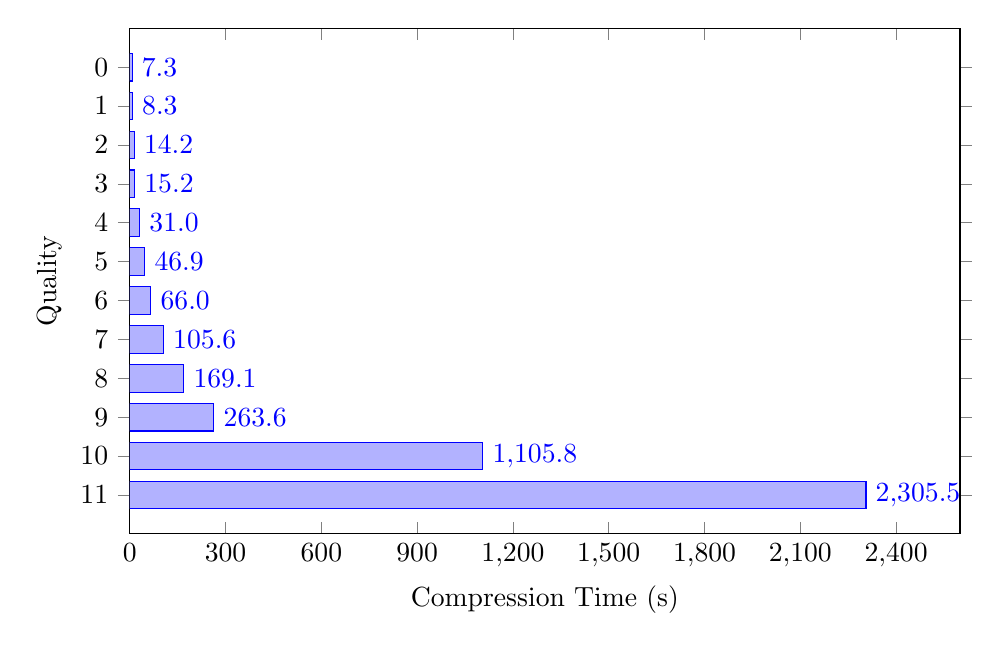
\begin{tikzpicture}
\begin{axis}[
	width = \textwidth,
	height = 1.1*\axisdefaultheight,
	xbar,
	xmin = 0,
	xmax = 2600,
	xtick distance = 300,
	y dir = reverse,
	ytick = data,
	scaled ticks = false,
	enlarge x limits = {abs = 0},
	enlarge y limits = {abs = 1},
	nodes near coords,
	nodes near coords align = {horizontal},
	nodes near coords style = {/pgf/number format/.cd, fixed zerofill, precision = 1},
	xlabel = Compression Time (s),
	ylabel = Quality
]
\addplot coordinates {
	(7.26, 0)
	(8.28, 1)
	(14.16, 2)
	(15.23, 3)
	(31.01, 4)
	(46.94, 5)
	(65.97, 6)
	(105.56, 7)
	(169.08, 8)
	(263.59, 9)
	(1105.75, 10)
	(2305.51, 11)
};
\end{axis}
\end{tikzpicture}